\documentclass[a4paper, 12pt]{article}
\usepackage{graphicx}
\graphicspath{{images/}}

\begin{document}
	\begin{center}
	\textbf{Modeling Assignment 1 : Variety Expansion Models}
	\linebreak
	\linebreak	
	\textbf{Kshitiz Dahal}
	\linebreak
	\linebreak
	
	ANR: 123934	
	\end{center}
	\newpage
	\begin{flushleft}
		\textbf{\textit{1.Introduction to the two Variety Expansion Models }}
	\end{flushleft}
	\begin{flushleft}
		\textit{a. Simple Variant of the Product-variety Model:} This model is built on the assumption that final output is used as an R\&D input. The intuition behind the model is that the final good is used for consumption and investment. Its only other use is in producing intermediate products. So, the economy's Gross Domestic Product (GDP) is final output	$ Y_t $ minus the amount used in intermediate production.
	\end{flushleft}
	\begin{flushleft}
		\textit{b.Romer Model with Labor as R\&D Input:} In this alternative model , a fraction of Labor, $ L_1 $ is used in the production of final goods, and the other fraction, $ L_2 $ is allocated for research activities directed towards increasing variety.
	\end{flushleft}
	\newpage
	\begin{center}
		\textbf{b.Comparison between two alternative Variety Expansion Models}
	\end{center}
	\begin{flushleft}
		The most fundamental difference between Model 1 and Model 2 comes from the source of input used for production of intermediate products (the R\&D input). A portion of output R is used as R\&D input in Model 1, whereas a fraction of Labor $ L_2 $ is the R\&D input in second model.
		
	\end{flushleft}
	\begin{flushleft}
		Because of the fundamental differences mentioned above, the first model has the whole Labor L in its output equation whereas, only $ L_1 $ is seen in Model 2 because the rest of the population $ L_2 $ is in R\&D instead of output production. Thus, the two models differ mostly in terms of the labor term.
	\end{flushleft}
	\newpage
	\begin{center}
		\textbf{Let's compare outputs in the two models}
		
\includegraphics{images/output}	
	\end{center}			

	\newpage
	\begin{flushleft}
		\textbf{Output}
	\end{flushleft}	
	\begin{flushleft}
		The final goods' output in Model 1 is given by:-
	\end{flushleft}
	\begin{center}
		$$ Y_t = L^{1-\alpha}\int_{0}^{M_t}x_i^{\alpha}dx$$
		\begin{flushleft}
			Or,
		\end{flushleft}
		\begin{center}
			$$Y_t = L^{1-\alpha} \sum_{i=1}^{M_t} x_i^{\alpha} $$
		\end{center}
	\end{center}

\begin{flushleft}
	The final goods' output in Model 2 is given by:-
\end{flushleft}
\begin{center}
	$$ Y_t = L_1^{1-\alpha}\int_{0}^{M_t}x_i^{\alpha}dx$$
	\begin{flushleft}
		Or,
	\end{flushleft}
	\begin{center}
		$$Y_t = (L-L_R)^{1-\alpha} \sum_{i=1}^{M_t} x_i^{\alpha} $$
	\end{center}
\end{center}
\newpage
\begin{flushleft}
	\textbf{Intermediate Products}
	\begin{flushleft}
		The amount of intermediate products used in Model 1 is given by :-
	\end{flushleft}
	\begin{center}
		$x = L \alpha ^ \frac {2} {1-\alpha}$
	\end{center}
	\begin{flushleft}
		Or,
	\end{flushleft}
	\begin{center}
		$ Y = (ML_y)^{1-\alpha} (s_x Y)^{\alpha} $
	\end{center}
		\begin{flushleft}
			The amount of intermediate products used in Model 2 is given by :-
		\end{flushleft}
		\begin{center}
			$x = L_1 \alpha ^ {\frac {2} {(1-\alpha)}}$
		\end{center}
		\begin{flushleft}
			Or,
		\end{flushleft}
		\begin{center}
			$ Y = M(L-L_R)s_x^ {\frac{\alpha}{(1-\alpha)}} $
		\end{center}
\end{flushleft}
\newpage
\begin{flushleft}
	\textbf{Rate of innovation}
	\begin{flushleft}
		The rate at which the variety expands, that is, the rate of innovation for Model 1 is given by :-
		\begin{center}
			$$ \frac{dM_t}{dt}=\lambda R_t $$
		\end{center}
		\begin{flushleft}
			Or,
		\end{flushleft}
		\begin{center}
			$\dot{M}=\lambda R  $
		\end{center}
	\end{flushleft}
	\begin{flushleft}
		The rate at which the variety expands, that is, the rate of innovation for Model 2 is given by :-
		\begin{center}
			$$ \frac{dM_t}{dt}=\lambda M_t L_2 $$
		\end{center}
		\begin{flushleft}
			Or,
		\end{flushleft}
		\begin{center}
			$\dot{M}=\lambda_L M L_R  $
		\end{center}
	\end{flushleft}
\end{flushleft}
\newpage
\begin{flushleft}
	\textbf{Profits}
	\begin{flushleft}
		The profits for innovation sector in Model 1 is given by:-
	\end{flushleft}
	\begin{center}
		$ \pi = \frac{1-\alpha}{\alpha}L \alpha^{\frac {2}{1-\alpha}} $
	\end{center}
	\begin{flushleft}
		The profits for innovation sector in Model 2 is given by:-
	\end{flushleft}
	\begin{center}
		$ \pi = \frac{1-\alpha}{\alpha}L_1 \alpha^{\frac {2}{1-\alpha}} $
	\end{center}
\end{flushleft}
\newpage
\begin{flushleft}
	\textbf{Interest rates}
	\begin{flushleft}
		The rate of return for Model 1 is given by :-
	\end{flushleft}
	\begin{center}
		$r = \lambda\alpha L(1-\alpha)s_x^{\frac{\alpha}{1-\alpha}}$
	\end{center}
		\begin{flushleft}
			The rate of return for Model 2 is given by :-
		\end{flushleft}
		\begin{center}
			$r = \lambda_L\alpha (L-\frac {g}{\lambda_L})$
		\end{center}
\end{flushleft}
\newpage
\begin{flushleft}
	\textbf{Growth Rate}
	\begin{flushleft}
			The growth rate for Model 1 is given by :-
	\end{flushleft}
	\begin{center}
		$$ g = \frac{\lambda \frac{1-\alpha} {\alpha} L\alpha^{\frac {2} {1-\alpha}}-\rho } {\varepsilon} $$
	\end{center}
	\begin{flushleft}
		The growth rate for Model 2 is given by :-
	\end{flushleft}
	\begin{center}
		$$ g = \frac{\alpha \lambda L - \rho}{\alpha + \varepsilon} $$
	\end{center}
\end{flushleft}
\newpage
\begin{center}
	\textbf{Graphical Representation}
	
	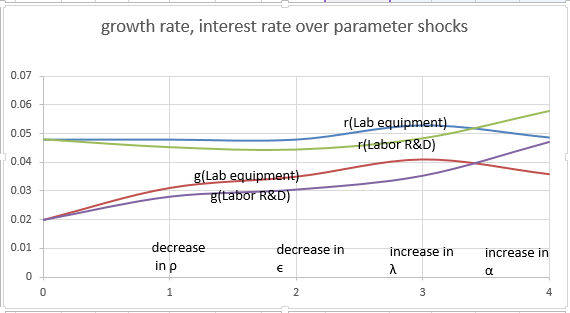
\includegraphics{images/ExcelGraph}
	
	Growth and interest rate in response to parameter shocks
\end{center}
\newpage
\begin{flushleft}
	\textbf{d. Comments from numerical calibration in Excel}
		\begin{flushleft}
			The effect of change in preferences $ (\rho $ and $ \varepsilon) $ showed following characteristics over the two models :-
		\end{flushleft}
		\begin{flushleft}
			\begin{itemize}
				\item Increasing growth rate needs more effort in Labor R\&D Model than Lab Equipment Model as shown by the response of growth rate to parameter shocks.
			\end{itemize}
			\begin{itemize}
				\item Returns on innovation (interest rates) are independent of growth rate for Lab Equipment Model whereas returns on innovation dropped in Labor R\&D Model when growth rates increased.
			\end{itemize}
			\begin{itemize}
				\item The response of growth rates to parameter shocks was as expected. The growth rates changed in the same direction.
			\end{itemize}
		\end{flushleft}
		\begin{flushleft}
			The effect of change in initial condition $(\lambda)$
			\begin{itemize}
				\item The growth rates changed in both directions, but the effect was bigger for Lab Equipment Model.
			\end{itemize}
		\end{flushleft}
		\begin{flushleft}
			The effect of change in $ \alpha $
			\begin{itemize}
				\item The change in $ \alpha $ changed the growth rates in different direction, decreasing growth rate for Lab Equipment Model, while increasing growth rate for Labor R\&D model.
			\end{itemize}
		\end{flushleft}
\end{flushleft}
\newpage
\begin{flushleft}
	\textbf{Conclusion}
	\begin{flushleft}
		\begin{itemize}
			\item The models behaved differently with respect to different parameter shocks because of the difference in inputs used for R\&D between two models.
			\item Both models have the prospects of unbounded growth 
		\end{itemize}
	\end{flushleft}
\end{flushleft}
\newpage
\begin{center}
	
	
	
\includegraphics{images/ThankYou}
	

\end{center}
	
\end{document}

